The Kaya decomposition presented in Section \ref{sec:decomposition} identifies $\text{CI}_{\text{elec}}$, the carbon intensity of electricity, as one of the most actionable levers for reducing CO$_2$ emissions from copper production. Unlike ore grade, which is a geological constraint, $\text{CI}_{\text{elec}}$ responds directly to energy policy and investment decisions. This has an important implication for electrification: replacing diesel and fossil fuels with electricity across the copper production chain only reduces emissions if the electricity itself is low-carbon. On a coal-heavy grid, electrification can actually worsen the carbon footprint, as indirect emissions from power generation may exceed the savings from cutting on-site combustion. This section examines why Chile is increasingly moving away from this risk, and why the conditions for productive electrification are now largely in place.

\subsection{Historical Evolution of the Electricity Mix}

\subsubsection{Geographic Foundations of the Energy Transition}

Chile's renewable energy potential is largely a product of its geography. The country stretches over 4,300~km from north to south, which places very different climatic zones within the same national grid.

\begin{figure}[H]
    \centering
    \begin{minipage}{0.48\textwidth}
        \centering
        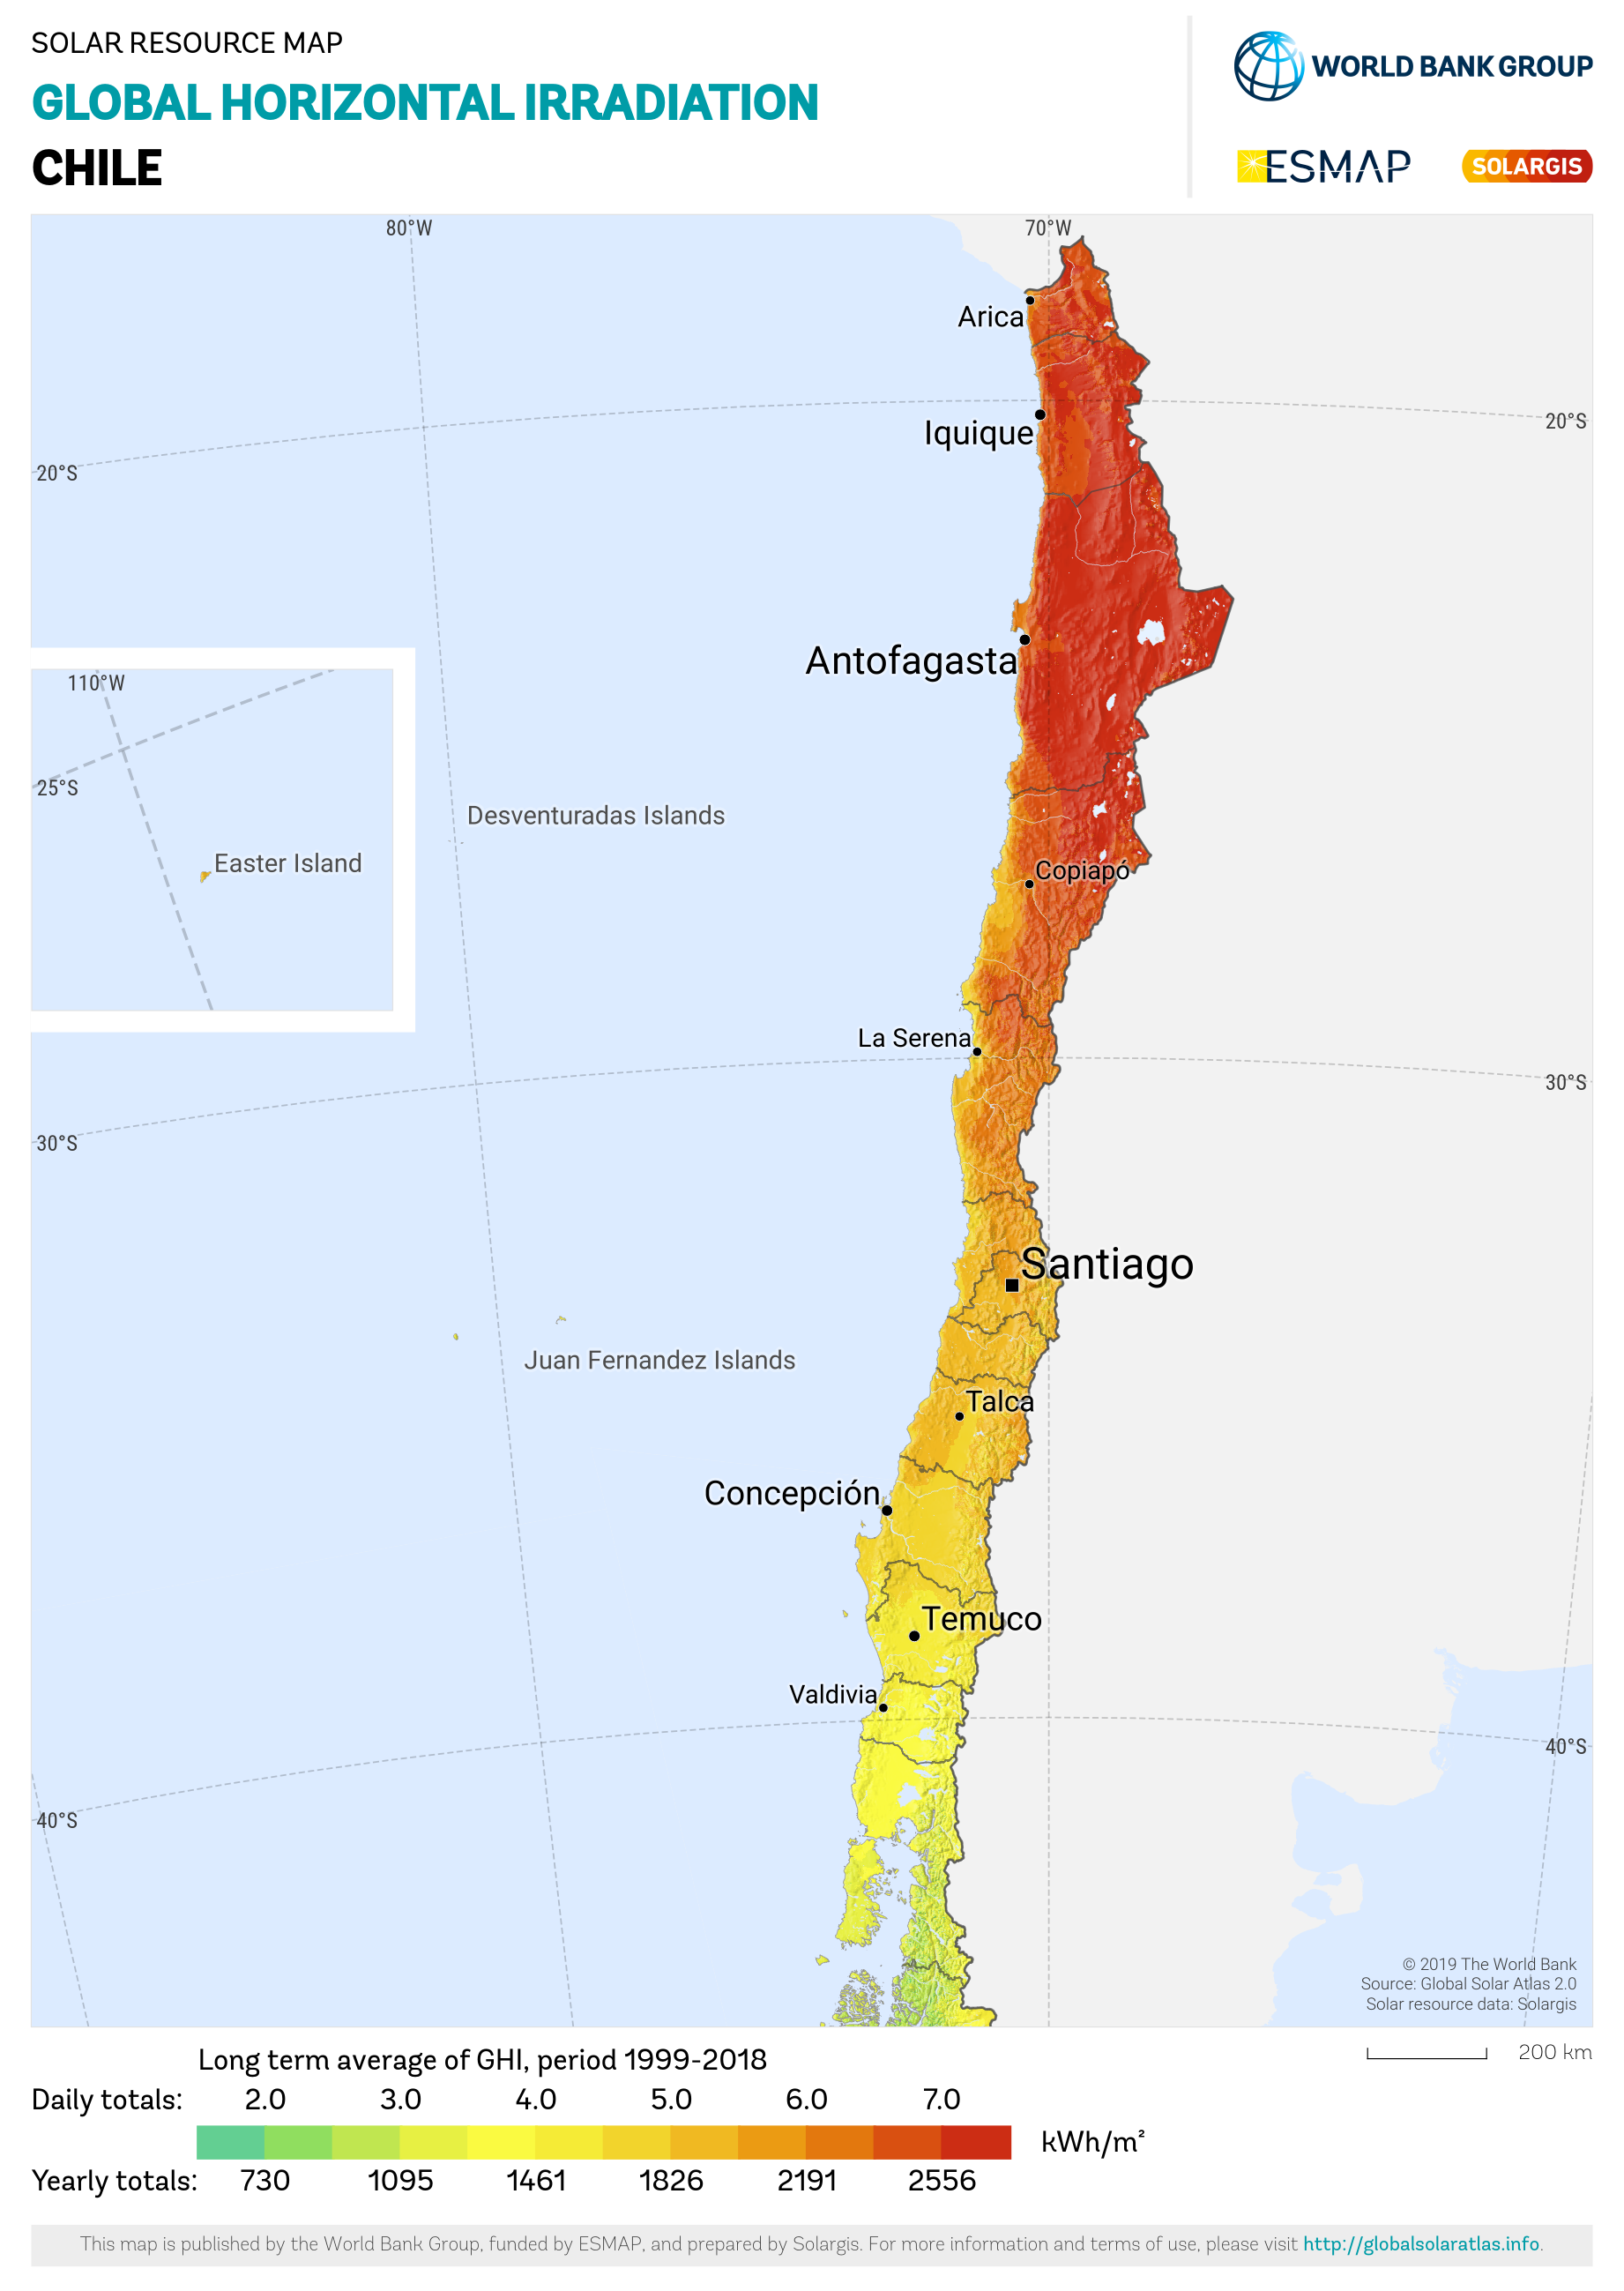
\includegraphics[width=\linewidth]{Figures/Chile_GHI_mid-size-map_156x220mm-300dpi_v20191015.png}
        \caption{Global Horizontal Irradiation (GHI) in Chile, long-term average 1999--2018 (kWh/m$^2$). \textcopyright~2019 The World Bank, Source: Global Solar Atlas~2.0, Solar resource data: Solargis.}
        \label{fig:ghi_map}
    \end{minipage}
    \hfill
    \begin{minipage}{0.48\textwidth}
        \centering
        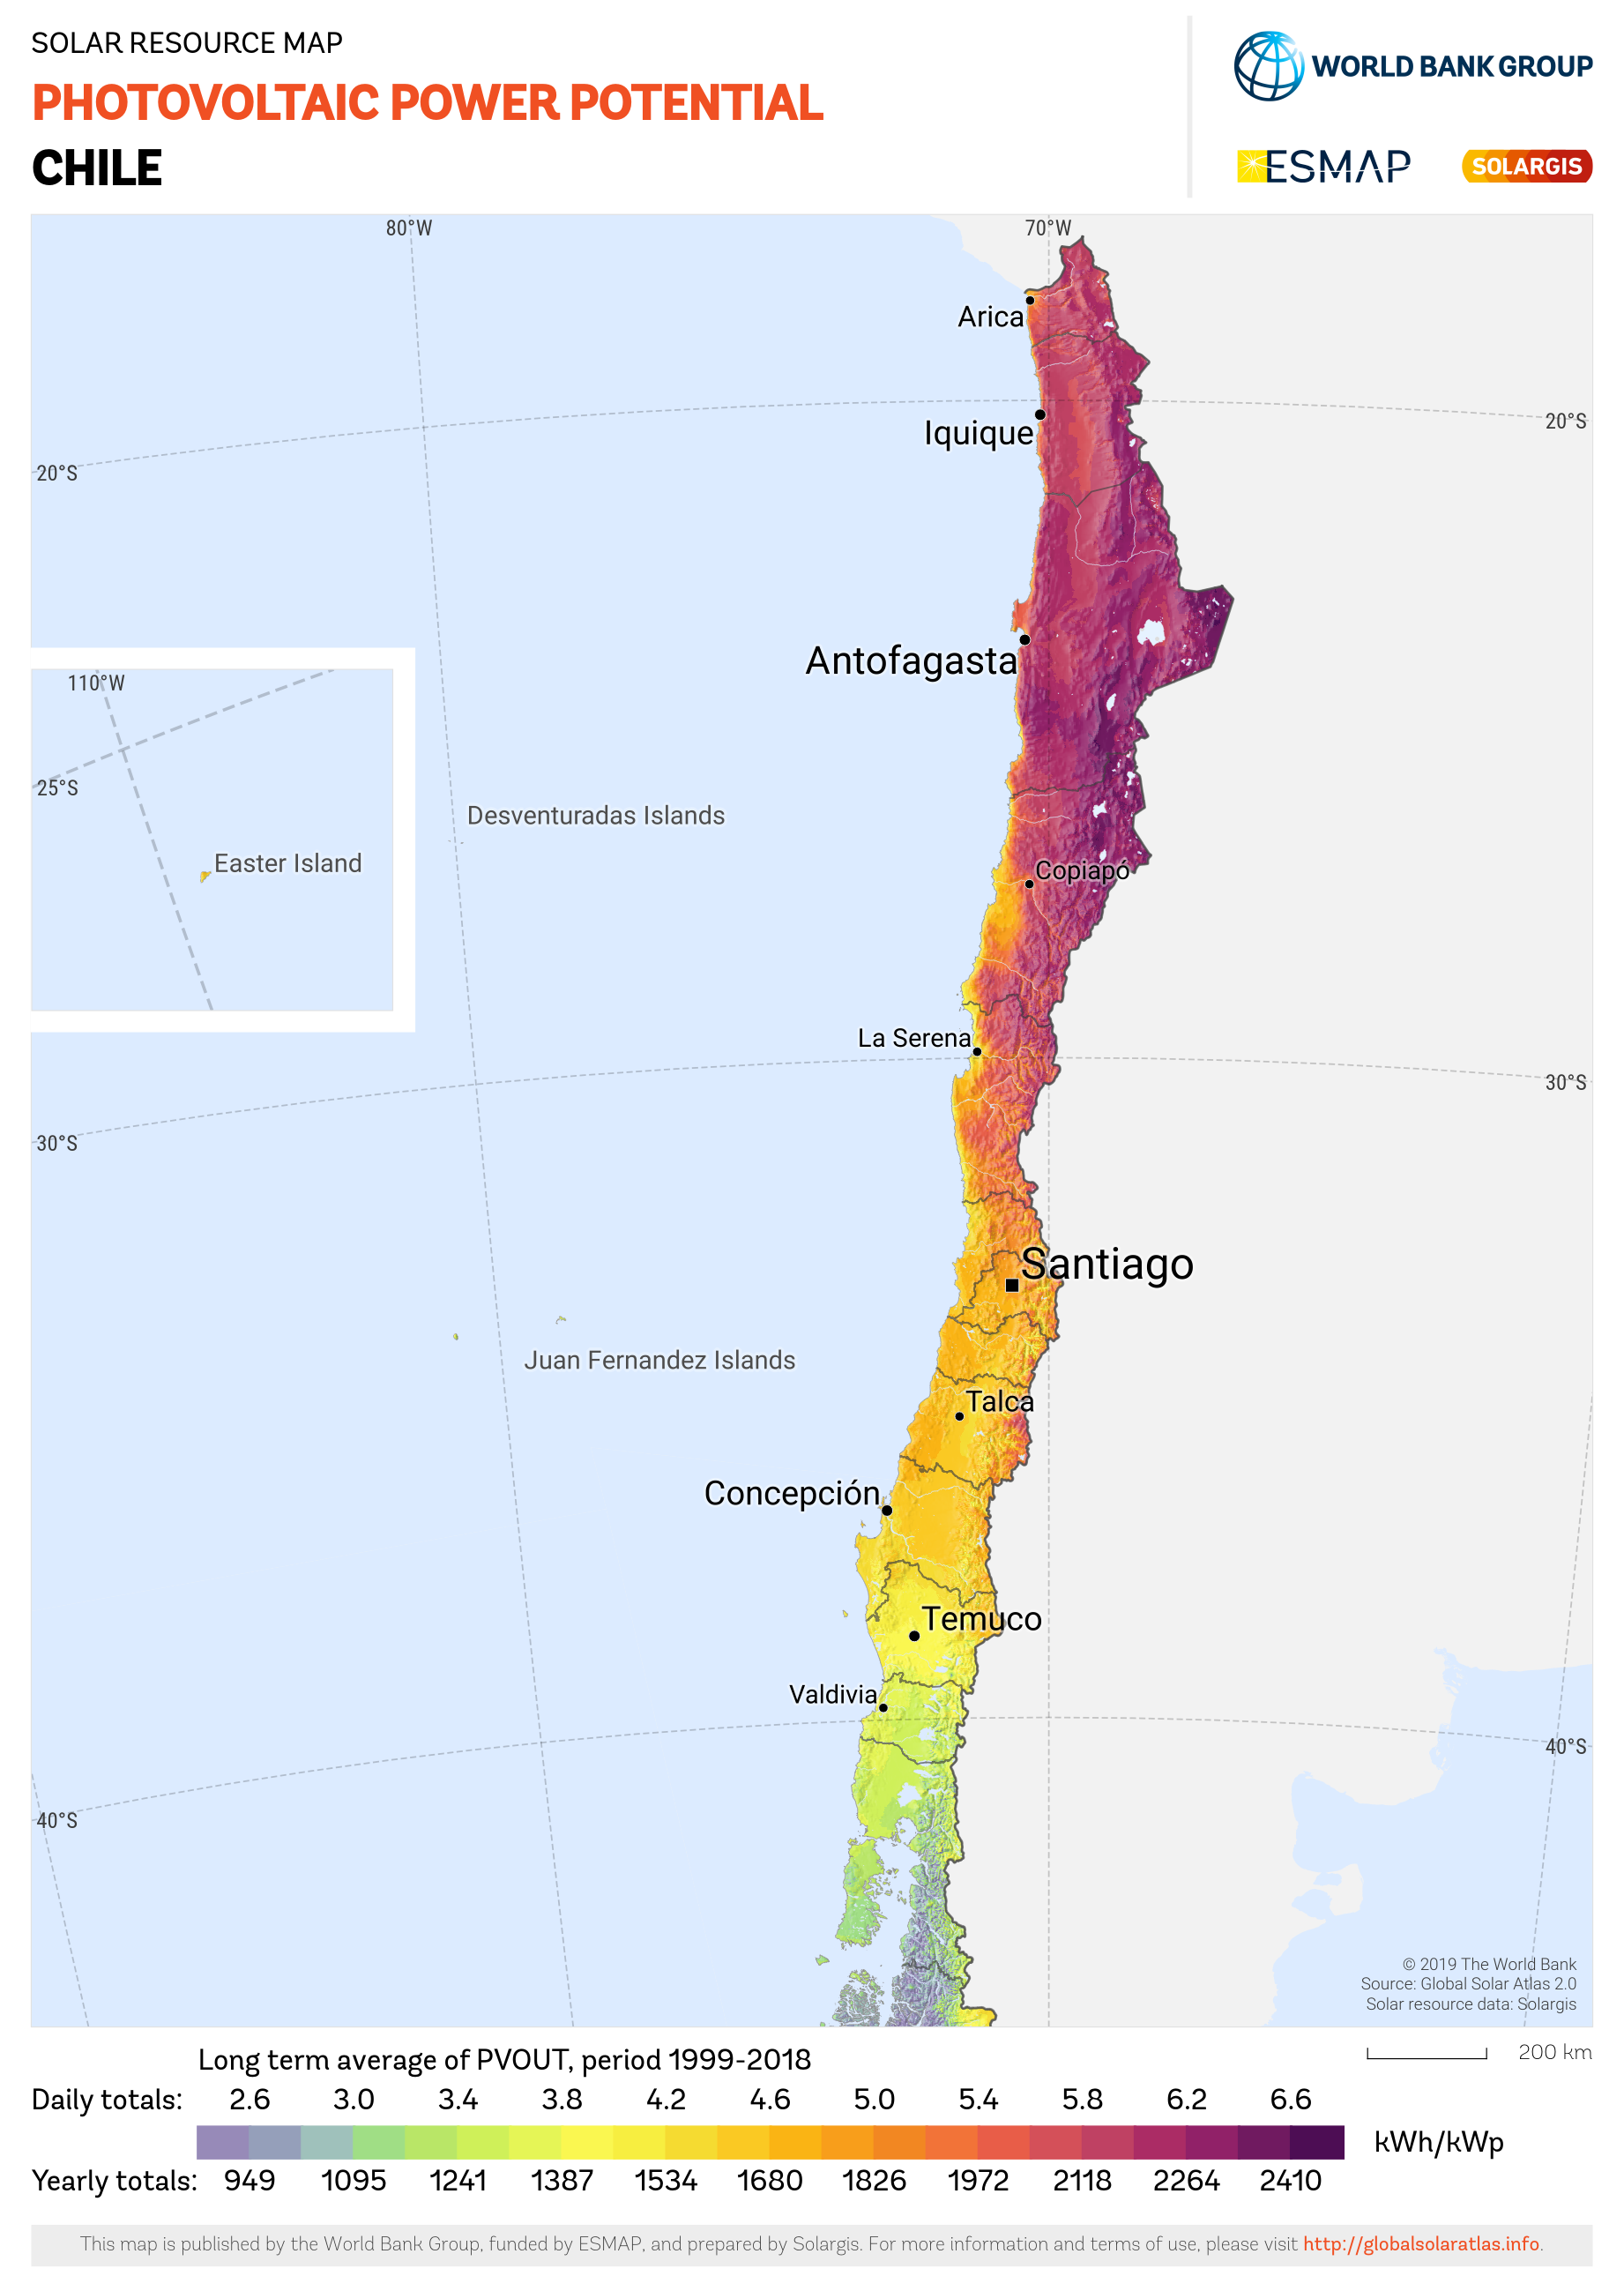
\includegraphics[width=\linewidth]{Figures/Chile_PVOUT_mid-size-map_156x220mm-300dpi_v20191015.png}
        \caption{Photovoltaic power potential (PVOUT) in Chile, long-term average 1999--2018 (kWh/kWp). \textcopyright~2019 The World Bank, Source: Global Solar Atlas~2.0, Solar resource data: Solargis.}
        \label{fig:pvout_map}
    \end{minipage}
\end{figure}

\begin{figure}[H]
    \centering
    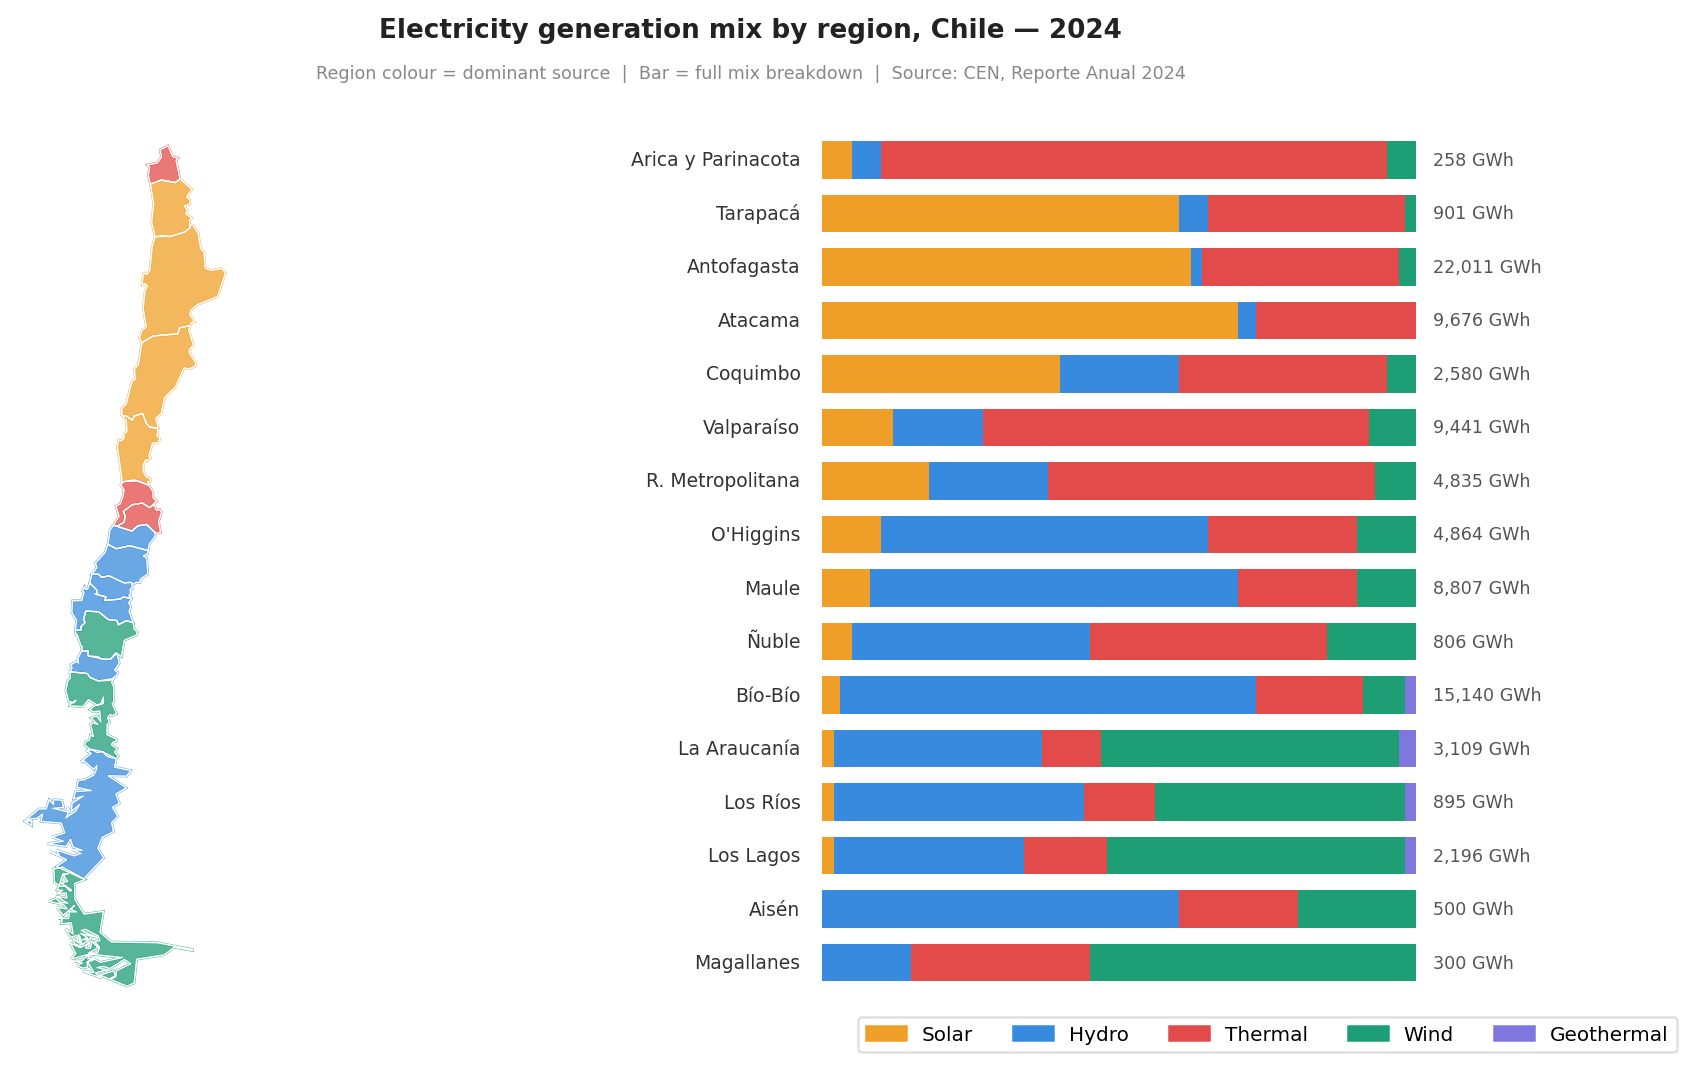
\includegraphics[width=0.72\linewidth]{Figures/chile_energy_map.png}
    \caption{Electricity generation mix by region in Chile, 2024. Each region is coloured by its dominant source; horizontal bars show the full breakdown, with output in GWh. Source: Coordinador Eléctrico Nacional, Reporte Anual 2024.}
    \label{fig:cen_region}
\end{figure}

As Figure~\ref{fig:cen_region} illustrates, Chile's geography creates three broadly distinct renewable energy zones \cite{SolarAtlas2019}. The northern desert, with Global Horizontal Irradiance values regularly exceeding 2,500~kWh/m$^2$/year, is dominated by solar photovoltaic. The central zone relies primarily on hydropower, drawing on the river systems fed by Andean snowmelt. The south benefits from strong and consistent winds, making it one of the most promising onshore wind corridors in the world. These three resources peak at different times of day and year, which makes them a good fit for each other within a single grid.

\subsubsection{From Coal Dominance to Renewable Leadership (2000--2024)}

Between 2000 and 2013, Chile expanded its coal-fired capacity to keep pace with rapid demand growth, and the carbon intensity of the grid rose accordingly, reaching approximately 482~gCO$_2$/kWh in 2013 \cite{IEAChile2024}. Coal still accounted for 43.6\% of electricity output as late as 2016 \cite{ProgressPlaybook2024}. The shift began around 2014--2015, when falling costs for solar PV and wind, combined with resistance from local communities to new thermal projects, started to alter the investment landscape. The pace of change accelerated after 2019, as shown in Figure~\ref{fig:owid_mix}.

\begin{figure}[H]
    \centering
    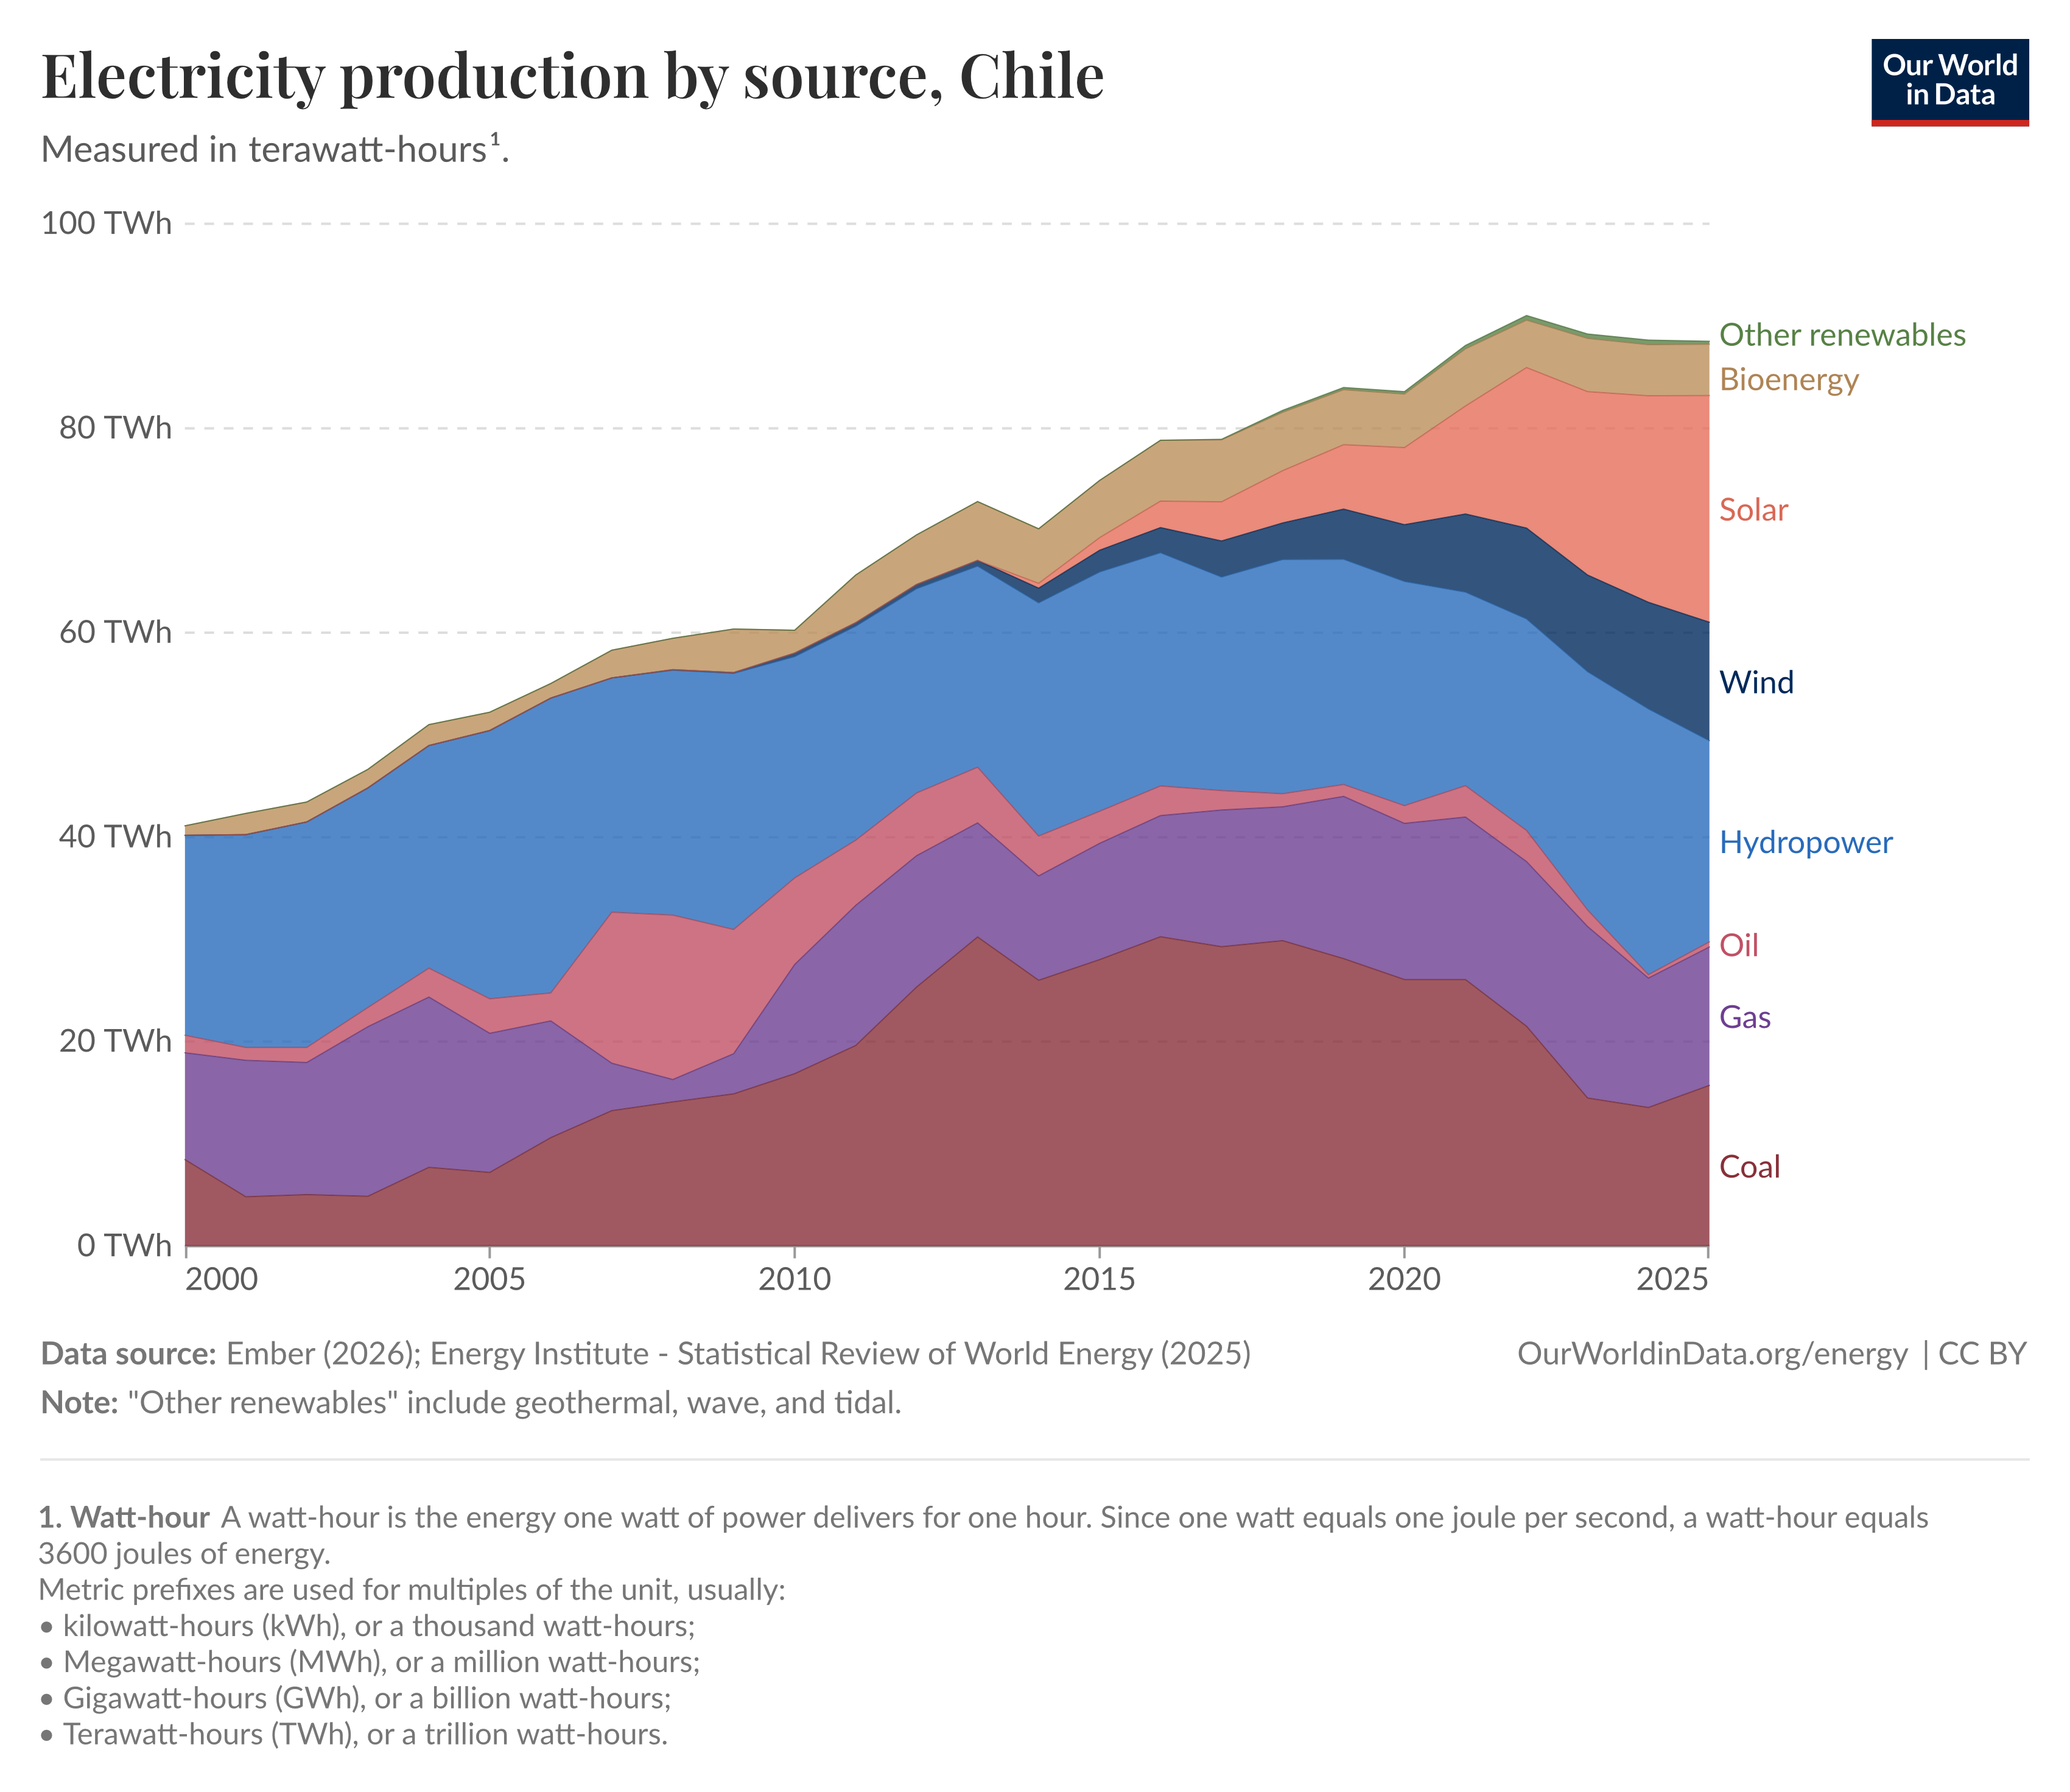
\includegraphics[width=0.85\linewidth]{Figures/electricity-prod-source-stacked.png}
    \caption{Electricity production by source in Chile, 2000--2025 (TWh). Source: Our World in Data, based on Ember (2026) and Energy Institute -- Statistical Review of World Energy (2025) \cite{OWID2026}.}
    \label{fig:owid_mix}
\end{figure}

By 2024, renewables accounted for roughly 70\% of national electricity generation, while coal had retreated to 14\% \cite{EnergiaEstrategica2025}. Solar and wind together provided 35\% of generation that year, compared to 14\% in 2019 \cite{Ember2025}. Solar energy alone reached 19.92~TWh, or 22.3\% of total national output, up from less than 0.1\% in 2013 \cite{WikipediaSolar2025}.

These shifts in the generation mix translated directly into a lower $\text{CI}_{\text{elec}}$. From IEA data on power sector emissions and total production, we compute that the carbon intensity of Chilean electricity fell from its 2013 peak of 482~gCO$_2$/kWh to 221~gCO$_2$/kWh in 2023, a reduction of over 54\% in ten years. The industry body Generadoras de Chile reports a consistent picture using the national grid emissions factor, which declined from 0.53~tCO$_2$/MWh in 2013 to 0.20~tCO$_2$/MWh in 2024, a 63\% drop over the same period. At the national level, energy-related CO$_2$ emissions peaked at 94~Mt in 2019 and had fallen by over 20\% to 72~Mt by 2024 \cite{IEAChile2026}.

\begin{figure}[H]
    \centering
    \begin{minipage}{0.48\textwidth}
        \centering
        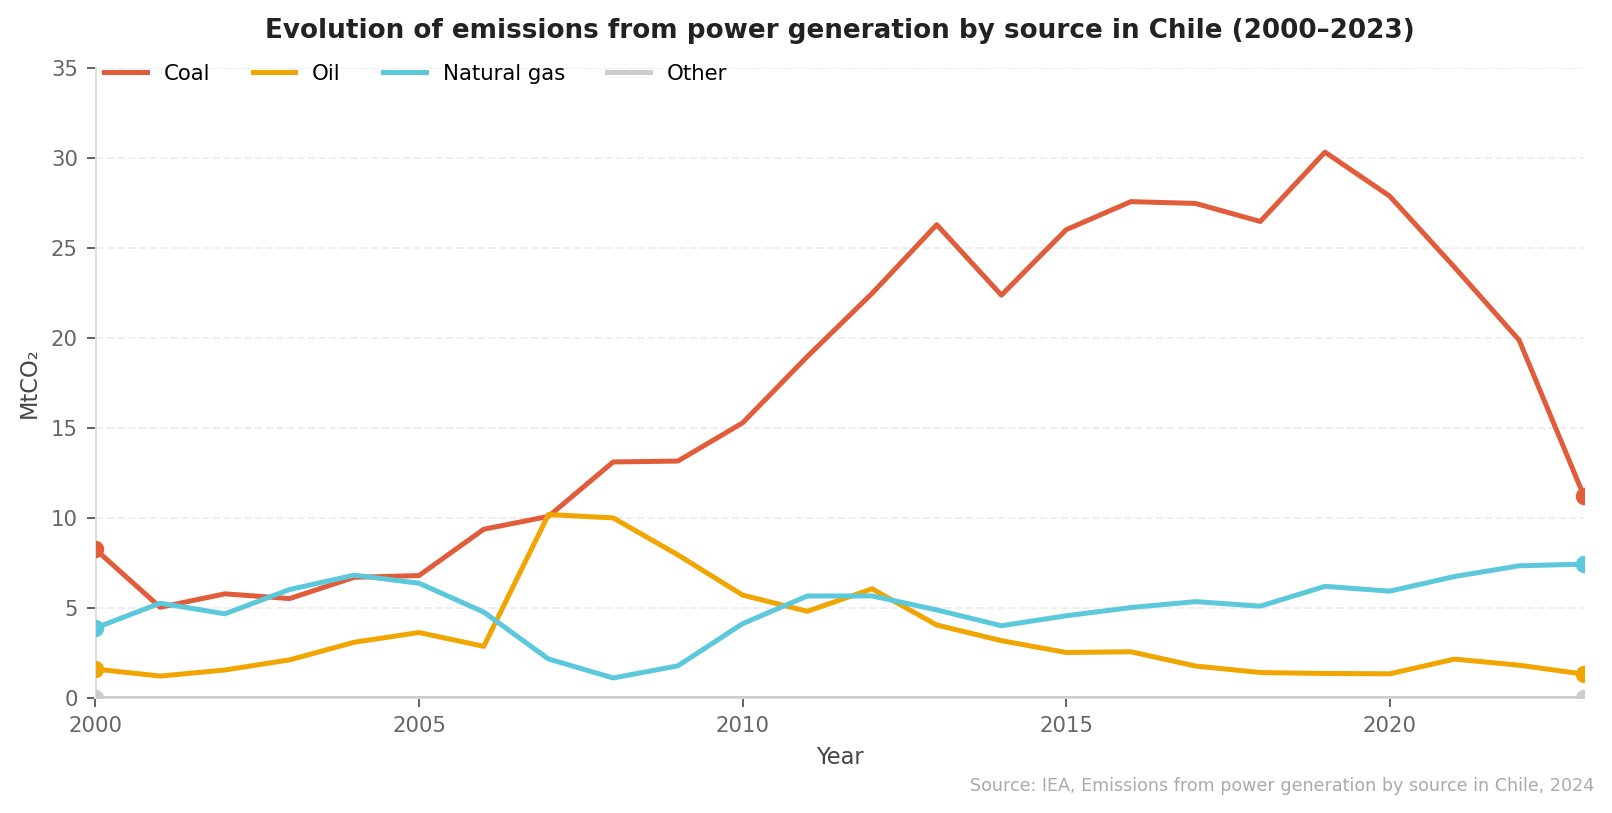
\includegraphics[width=\linewidth]{Figures/chile_emissions_by_source.png}
        \caption{CO$_2$ emissions from power generation by source in Chile, 2000--2023 (MtCO$_2$). Source: IEA, authors' calculations.}
        \label{fig:emissions_source}
    \end{minipage}
    \hfill
    \begin{minipage}{0.48\textwidth}
        \centering
        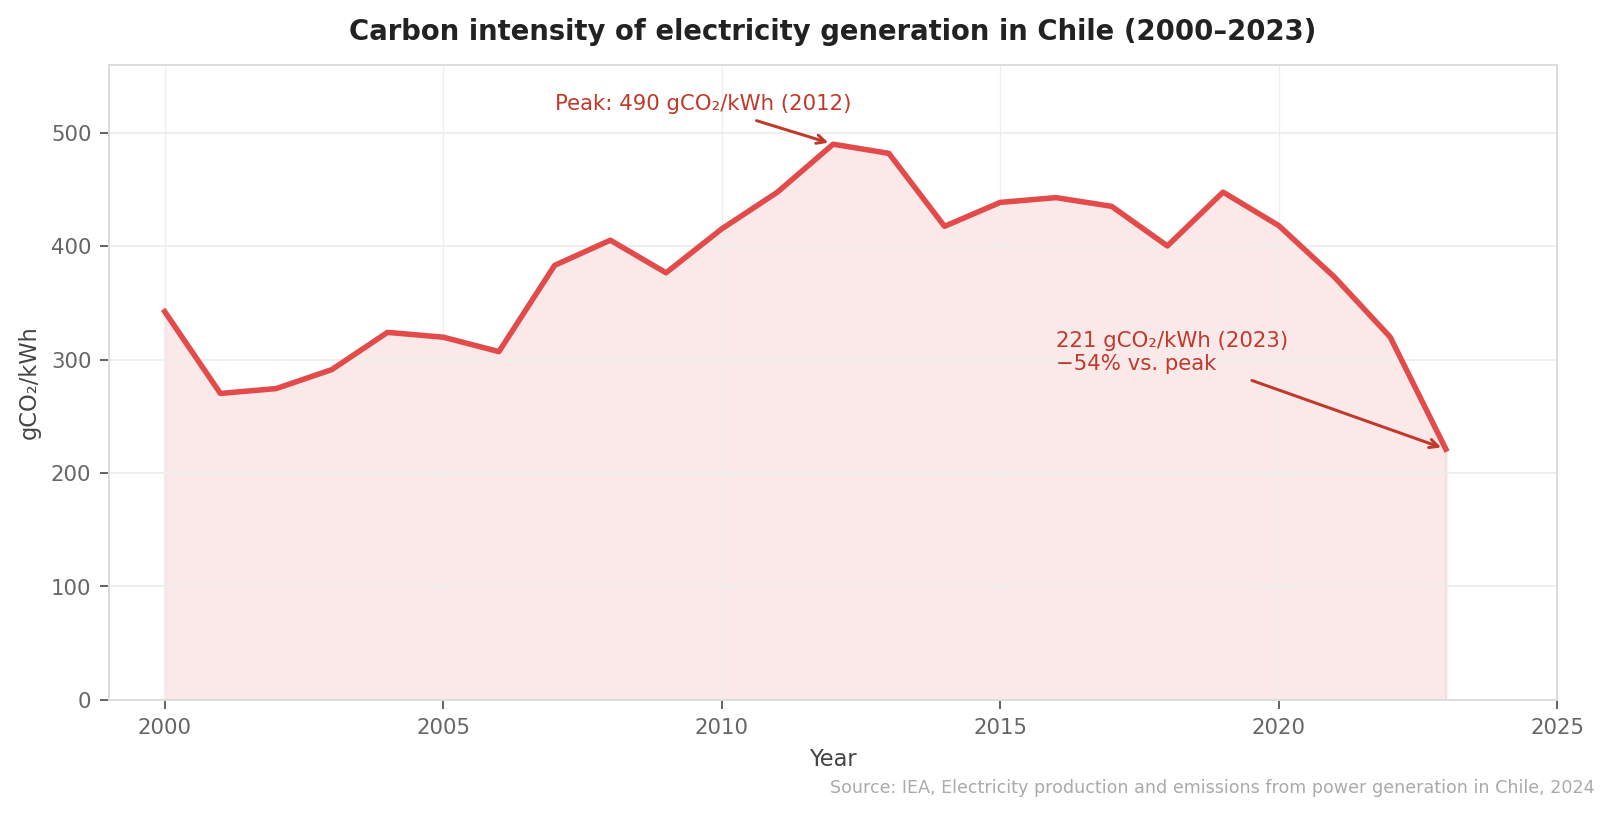
\includegraphics[width=\linewidth]{Figures/chile_ci_elec.png}
        \caption{Carbon intensity of electricity generation in Chile, 2000--2023 (gCO$_2$/kWh). Source: IEA, authors' calculations.}
        \label{fig:ci_elec}
    \end{minipage}
\end{figure}

Figures~\ref{fig:emissions_source} and~\ref{fig:ci_elec} show the same trend from two angles. The fall in coal-fired generation cut the grid's carbon intensity roughly in half, from a peak of 482~gCO$_2$/kWh in 2013 to 221~gCO$_2$/kWh in 2023. On the capacity side, eleven coal plants have been retired since 2018, removing 1,679~MW from the grid, while over 19,000~MW of renewable generation and storage capacity have been added over the same period. As of November 2024, ERNC capacity totalled 16,422~MW in the SEN, representing 47.4\% of total installed capacity across all national electricity systems \cite{CNE2024}. Solar PV accounts for 29.9\% of this total and wind for 13.6\%, with both technologies still expanding rapidly.

\subsection{Political Commitments and Legal Framework}

Chile's energy transition is backed by a fairly solid legal and political framework. In 2020, Chile submitted an updated Nationally Determined Contribution (NDC) to the UNFCCC, committing to cap greenhouse gas emissions at 95~MtCO$_2$e by 2030 and to peak emissions no later than 2025, with a binding objective of carbon neutrality by 2050 \cite{CAT2020}. The Climate Action Tracker rates Chile's overall targets as ``Almost Sufficient'', meaning the ambition is above average by international standards but still falls short of full alignment with the 1.5°C pathway.

On the electricity side, the government has been more concrete. Since 2018, eleven coal plants have been voluntarily shut down under agreements between the government and the main utilities, ahead of any legal requirement to do so. A broader coal phase-out by 2040 is now government policy, with proposals circulating to bring that deadline forward to 2035, and the Energy Transition Act passed in December 2024 strengthens the legal basis for accelerating renewable deployment and integrating storage into the grid \cite{GLI2026}.

For copper mining, these commitments are particularly relevant: the sector consumes close to 30\% of Chile's national electricity \cite{Cochilco2024}, so any drop in the grid's carbon intensity reduces mining emissions automatically, even before any changes are made at the mine level.

\subsection{Projections and Implications for Copper Electrification}

According to the IEA's 2050 Energy Transition Roadmap for Chile, the carbon intensity of the grid is expected to fall from around 189~gCO$_2$/kWh today to 29~gCO$_2$/kWh by 2035, as coal is phased out and renewables continue to expand. As shown in Figure~\ref{fig:ci_elec_proj}, this would represent a reduction of over 85\% compared to the 2013 peak.

\begin{figure}[H]
    \centering
    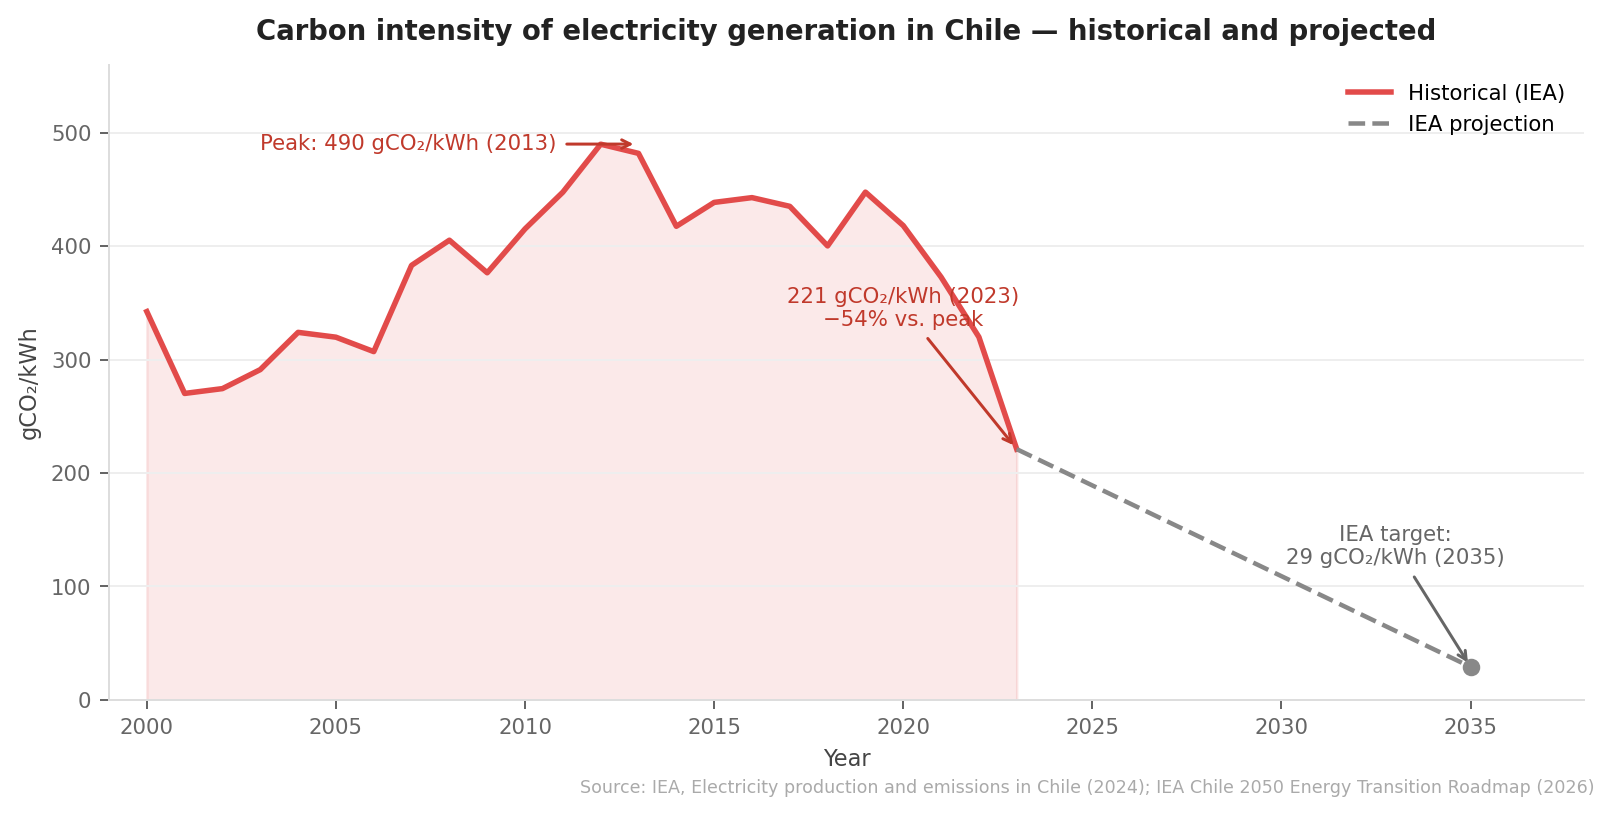
\includegraphics[width=0.85\linewidth]{Figures/chile_ci_elec_projection.png}
    \caption{Carbon intensity of electricity generation in Chile, historical and projected (gCO$_2$/kWh). Source: IEA.}
    \label{fig:ci_elec_proj}
\end{figure}

At 29~gCO$_2$/kWh, the indirect emissions from grid electricity become small compared to the direct emissions from burning diesel or gas on-site. Electrifying operations such as haulage, crushing, or concentration would then produce real emission reductions rather than simply shifting them from one source to another. The grid is already clean enough to make this worthwhile, and the trend is set to continue.